\setlength{\columnsep}{3pt}
\begin{flushleft}
	\bigskip
	\begin{itemize}
		\item RPM is a collection of different files that constitues a package.
		\item RPM stands for \textbf{Red Hat Package Manager}.
		\item It was developed by Red Hat company.
		\item RPM is used on Red Hat-based Linux operating systems (like Fedora, CentOS, RHEL, etc.)
		\item An RPM package uses the \textbf{.rpm} extension.

		\bigskip
		\item Syntax of package name:
		\begin{figure}[h!]
			\centering
			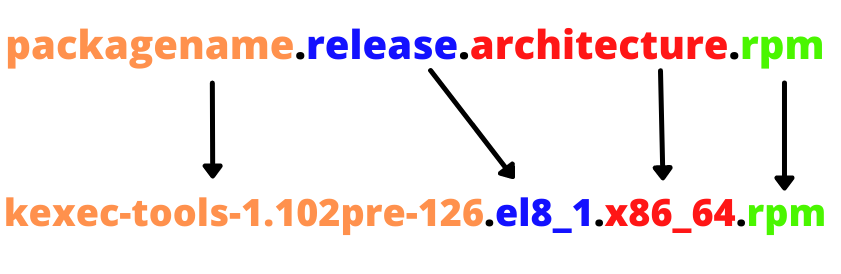
\includegraphics[scale=.5]{content/chapter11/images/package2.png}
			\caption{Package name syntax}
			\label{fig:package_name}
		\end{figure}
	\end{itemize}
\end{flushleft}
\newpage


